% Judul dokumen
\title{Buku Tugas Akhir ITS}
\author{Musk, Elon Reeve}

% Pengaturan ukuran teks dan bentuk halaman dua sisi
\documentclass[12pt,twoside]{report}

% Pengaturan ukuran halaman dan margin
\usepackage[a4paper,top=30mm,left=30mm,right=20mm,bottom=25mm]{geometry}

% Pengaturan ukuran spasi
\usepackage[singlespacing]{setspace}

% Pengaturan detail pada file PDF
\usepackage[pdfauthor={\@author},bookmarksnumbered,pdfborder={0 0 0}]{hyperref}

% Pengaturan jenis karakter
\usepackage[utf8]{inputenc}

% Pengaturan pewarnaan
\usepackage[table,xcdraw]{xcolor}

% Pengaturan kutipan artikel
\usepackage[style=ieee, backend=biber]{biblatex}

% Package lainnya
\usepackage{changepage}
\usepackage{enumitem}
\usepackage{eso-pic}
\usepackage{etoolbox}
\usepackage{graphicx}
\usepackage{amsmath}
\usepackage{amssymb}
\usepackage{physics}
\usepackage{txfonts} % Font times
\usepackage{lipsum}
\usepackage{longtable}
\usepackage{tabularx}
\usepackage{wrapfig}
\usepackage{float}

\usepackage{tikz}
\usepackage{relsize}
\usetikzlibrary{shapes.geometric, arrows}

\tikzstyle{startstop} = [ellipse, minimum width=3cm, minimum height=1cm, text centered, draw=black, fill=red!30]
\tikzstyle{connector} = [circle, minimum width=1cm, minimum height=1cm, text centered, draw=black, fill=green!30]
\tikzstyle{io} = [trapezium, trapezium left angle=70, trapezium right angle=110, minimum width=1.5cm, minimum height=1cm, 
                  text centered, text width=2.5cm, draw=black, fill=blue!30]
\tikzstyle{io2} = [trapezium, trapezium left angle=70, trapezium right angle=110, minimum width=1.5cm, minimum height=1cm, 
                  text centered, text width=4cm, draw=black, fill=blue!30]
\tikzstyle{process} = [rectangle, minimum width=3cm, minimum height=1cm, text centered, text width=4cm, draw=black, fill=orange!30]
\tikzstyle{decision} = [diamond, aspect=2, minimum width=3cm,  minimum height=1cm, inner sep=0, text centered, text width=3cm, draw=black, fill=yellow!30]
\tikzstyle{arrow} = [thick,->,>=stealth]

% Definisi untuk "Hati ini sengaja dikosongkan"
\patchcmd{\cleardoublepage}{\hbox{}}{
  \thispagestyle{empty}
  \vspace*{\fill}
  \begin{center}\textit{[Halaman ini sengaja dikosongkan]}\end{center}
  \vfill}{}{}

% Pengaturan penomoran halaman
\usepackage{fancyhdr}
\fancyhf{}
\renewcommand{\headrulewidth}{0pt}
\pagestyle{fancy}
\fancyfoot[LE,RO]{\thepage}
\patchcmd{\chapter}{plain}{fancy}{}{}
\patchcmd{\chapter}{empty}{plain}{}{}

% Command untuk bulan
\newcommand{\MONTH}{%
  \ifcase\the\month
  \or Januari% 1
  \or Februari% 2
  \or Maret% 3
  \or April% 4
  \or Mei% 5
  \or Juni% 6
  \or Juli% 7
  \or Agustus% 8
  \or September% 9
  \or Oktober% 10
  \or November% 11
  \or Desember% 12
  \fi}
\newcommand{\ENGMONTH}{%
  \ifcase\the\month
  \or January% 1
  \or February% 2
  \or March% 3
  \or April% 4
  \or May% 5
  \or June% 6
  \or July% 7
  \or August% 8
  \or September% 9
  \or October% 10
  \or November% 11
  \or December% 12
  \fi}

% Pengaturan format judul bab
\usepackage{titlesec}
\titleformat{\chapter}[display]{\bfseries\Large}{BAB \centering\Roman{chapter}}{0ex}{\vspace{0ex}\centering}
\titleformat{\section}{\bfseries\large}{\MakeUppercase{\thesection}}{1ex}{\vspace{1ex}}
\titleformat{\subsection}{\bfseries\large}{\MakeUppercase{\thesubsection}}{1ex}{}
\titleformat{\subsubsection}{\bfseries\large}{\MakeUppercase{\thesubsubsection}}{1ex}{}
\titlespacing{\chapter}{0ex}{0ex}{4ex}
\titlespacing{\section}{0ex}{1ex}{0ex}
\titlespacing{\subsection}{0ex}{0.5ex}{0ex}
\titlespacing{\subsubsection}{0ex}{0.5ex}{0ex}

% Atur variabel berikut sesuai namanya

% nama
\newcommand{\name}{Aldifahmi Sihotang}
\newcommand{\authorname}{Sihotang, Aldifahmi}
\newcommand{\nickname}{Aldi}
\newcommand{\advisor}{Dr. Eko Mulyanto Yuniarno, S.T., M.T}
\newcommand{\coadvisor}{}
\newcommand{\examinerone}{}
\newcommand{\examinertwo}{}
\newcommand{\examinerthree}{}
\newcommand{\headofdepartment}{}

% identitas
\newcommand{\nrp}{0721 18 4000 0039}
\newcommand{\advisornip}{19680601 1995121 1 009}
\newcommand{\coadvisornip}{}
\newcommand{\examineronenip}{}
\newcommand{\examinertwonip}{}
\newcommand{\examinerthreenip}{}
\newcommand{\headofdepartmentnip}{}

% judul
\newcommand{\tatitle}{PENGEMBANGAN KURSI RODA OTONOM DENGAN \emph{ESP32-CAM} BERBASIS \emph{YOLOv8}}
\newcommand{\engtatitle}{\emph{DEVELOPMENT OF AUTONOMOUS WHEELCHAIR WITH ESP32-CAM BASED ON YOLOv8}}

% tempat
\newcommand{\place}{Surabaya}

% jurusan
\newcommand{\studyprogram}{Teknik Komputer}
\newcommand{\engstudyprogram}{Computer Engineering}

% fakultas
\newcommand{\faculty}{Teknologi Elektro dan Informatika Cerdas}
\newcommand{\engfaculty}{Intelligent Electrical and Informatics Technology}

% singkatan fakultas
\newcommand{\facultyshort}{FTEIC}
\newcommand{\engfacultyshort}{F-ELECTICS}

% departemen
\newcommand{\department}{Teknik Komputer}
\newcommand{\engdepartment}{Computer Engineering}

% kode mata kuliah
\newcommand{\coursecode}{TD123456}


% Tambahkan format tanda hubung yang benar di sini
\hyphenation{
  ro-ket
  me-ngem-bang-kan
  per-hi-tu-ngan
  tek-no-lo-gi
  me-la-ku-kan
  ber-so-si-al-i-sa-si
  pe-rang-kat
}

% Menambahkan resource daftar pustaka
\addbibresource{pustaka/pustaka.bib}

% Pengaturan format potongan kode
\usepackage{listings}
\definecolor{comment}{RGB}{0,128,0}
\definecolor{string}{RGB}{255,0,0}
\definecolor{keyword}{RGB}{0,0,255}
\lstdefinestyle{codestyle}{
  commentstyle=\color{comment},
  stringstyle=\color{string},
  keywordstyle=\color{keyword},
  basicstyle=\footnotesize\ttfamily,
  numbers=left,
  numberstyle=\tiny,
  numbersep=5pt,
  frame=lines,
  breaklines=true,
  prebreak=\raisebox{0ex}[0ex][0ex]{\ensuremath{\hookleftarrow}},
  showstringspaces=false,
  upquote=true,
  tabsize=2,
}
\lstset{style=codestyle}

% Isi keseluruhan dokumen
\begin{document}

% Sampul luar Bahasa Indonesia
\newcommand\covercontents{sampul/konten-id.tex}
\AddToShipoutPictureBG*{
  \AtPageLowerLeft{
    % Ubah nilai berikut jika posisi horizontal background tidak sesuai
    \hspace{-3.5mm}

    % Ubah nilai berikut jika posisi vertikal background tidak sesuai
    \raisebox{0mm}{
      
\includegraphics[width=\paperwidth,height=\paperheight]{sampul/gambar/sampul-luar.png}
    }
  }
}

% Menyembunyikan nomor halaman
\thispagestyle{empty}

% Pengaturan margin untuk menyesuaikan konten sampul
\newgeometry{
  top=95mm,
  left=25mm,
  right=20mm,
  bottom=25mm
}

\begin{flushleft}

  % Pemilihan font sans serif
  \sffamily

  % Pemilihan warna font putih
  \color{white}

  % Pemilihan font bold
  \fontseries{bx}
  \selectfont

  \input{\covercontents}

\end{flushleft}

\restoregeometry


% Atur ulang penomoran halaman
\setcounter{page}{1}

% Sampul dalam Bahasa Indonesia
\renewcommand\covercontents{sampul/konten-id.tex}
\AddToShipoutPictureBG*{
  \AtPageLowerLeft{
    % Ubah nilai berikut jika posisi horizontal background tidak sesuai
    \hspace{-4mm}

    % Ubah nilai berikut jika posisi vertikal background tidak sesuai
    \raisebox{0mm}{
      
\includegraphics[width=\paperwidth,height=\paperheight]{sampul/gambar/sampul-luar-tipis.png}
    }
  }
}

% Menyembunyikan nomor halaman
\thispagestyle{empty}

% Pengaturan margin untuk menyesuaikan konten sampul
\newgeometry{
  top=65mm,
  left=30mm,
  right=30mm,
  bottom=20mm
}

\begin{flushleft}

  % Pemilihan font sans serif
  \sffamily

  % Pemilihan font bold
  \fontseries{bx}
  \selectfont
  \begin{spacing}{1.5}
    \input{\covercontents}
  \end{spacing}

\end{flushleft}

\restoregeometry

\clearpage
\cleardoublepage

% Sampul dalam Bahasa Inggris
\renewcommand\covercontents{sampul/konten-en.tex}
\AddToShipoutPictureBG*{
  \AtPageLowerLeft{
    % Ubah nilai berikut jika posisi horizontal background tidak sesuai
    \hspace{-4mm}

    % Ubah nilai berikut jika posisi vertikal background tidak sesuai
    \raisebox{0mm}{
      
\includegraphics[width=\paperwidth,height=\paperheight]{sampul/gambar/sampul-luar-tipis.png}
    }
  }
}

% Menyembunyikan nomor halaman
\thispagestyle{empty}

% Pengaturan margin untuk menyesuaikan konten sampul
\newgeometry{
  top=65mm,
  left=30mm,
  right=30mm,
  bottom=20mm
}

\begin{flushleft}

  % Pemilihan font sans serif
  \sffamily

  % Pemilihan font bold
  \fontseries{bx}
  \selectfont
  \begin{spacing}{1.5}
    \input{\covercontents}
  \end{spacing}

\end{flushleft}

\restoregeometry

\cleardoublepage

% Label tabel dan gambar dalam bahasa indonesia
\renewcommand{\figurename}{Gambar}
\renewcommand{\tablename}{Tabel}

% Pengaturan ukuran indentasi paragraf
\setlength{\parindent}{2em}

% Pengaturan ukuran spasi paragraf
\setlength{\parskip}{1ex}

% Lembar pengesahan
\begin{center}
  \large
  \textbf{LEMBAR PENGESAHAN}
\end{center}

% Menyembunyikan nomor halaman
\thispagestyle{empty}

\begin{center}
  % Ubah kalimat berikut dengan judul tugas akhir
  \textbf{KALKULASI ENERGI PADA ROKET LUAR ANGKASA BERBASIS \emph{ANTI-GRAVITASI}}
\end{center}

\begingroup
% Pemilihan font ukuran small
\small

% \vspace{3ex}

\begin{center}
  \textbf{TUGAS AKHIR}
  \\Diajukan untuk memenuhi salah satu syarat memperoleh gelar Sarjana Teknik pada Program Studi S-1 Teknik Komputer Departemen Teknik Komputer Fakultas Teknologi Elektro dan Informatika Cerdas Institut Teknologi Sepuluh Nopember
\end{center}

% \vspace{3ex}

\begin{center}
  % Ubah kalimat berikut dengan nama dan NRP mahasiswa
  Oleh: \name{}
  \\NRP. \nrp{}
\end{center}

% \vspace{3ex}

% \begin{center}
% Ubah kalimat-kalimat berikut dengan tanggal ujian dan periode wisuda
%   Tanggal Ujian : 1 Juni 2021\\
%   Periode Wisuda : September 2021
% \end{center}

\begin{center}
  Disetujui oleh Tim Penguji Tugas Akhir:
\end{center}

% \vspace{4ex}

\begingroup
% Menghilangkan padding
\setlength{\tabcolsep}{0pt}

\noindent
\begin{tabularx}{\textwidth}{X l}
  % Ubah kalimat-kalimat berikut dengan nama dosen pembimbing pertama
  \advisor{}                       & (Pembimbing I)                      \\
  NIP: \advisornip{}               &                                     \\
                                   & ................................... \\
                                   &                                     \\
                                   &                                     \\
  % Ubah kalimat-kalimat berikut dengan nama dosen pembimbing kedua
  \coadvisor{}                     & (Pembimbing II)                     \\
  NIP: \coadvisornip{}             &                                     \\
                                   & ................................... \\
                                   &                                     \\
                                   &                                     \\
  % Ubah kalimat-kalimat berikut dengan nama dosen penguji pertama
  Dr. Galileo Galilei, S.T., M.Sc. & (Penguji I)                         \\
  NIP: 18560710 194301 1 001       &                                     \\
                                   & ................................... \\
                                   &                                     \\
                                   &                                     \\
  % Ubah kalimat-kalimat berikut dengan nama dosen penguji kedua
  Friedrich Nietzsche, S.T., M.Sc. & (Penguji II)                        \\
  NIP: 18560710 194301 1 001       &                                     \\
                                   & ................................... \\
                                   &                                     \\
                                   &                                     \\
  % Ubah kalimat-kalimat berikut dengan nama dosen penguji ketiga
  Alan Turing, ST., MT.            & (Penguji III)                       \\
  NIP: 18560710 194301 1 001       &                                     \\
                                   & ................................... \\
                                   &                                     \\
                                   &                                     \\
\end{tabularx}
\endgroup

% \vspace{2ex}

\begin{center}
  % Ubah kalimat berikut dengan jabatan kepala departemen
  Mengetahui, \\
  Kepala Departemen \department{} \facultyshort{} - ITS\\

  \vspace{8ex}

  % Ubah kalimat-kalimat berikut dengan nama dan NIP kepala departemen
  \underline{Dr. Supeno Mardi Susiki Nugroho, S.T., M.T.} \\
  NIP. 19700313 199512 1 001
\end{center}

\begin{center}
  \textbf{\MakeUppercase{\place{}}\\Bulan, \the\year{}}
\end{center}
\endgroup

\cleardoublepage
\begin{center}
  \large
  \textbf{APPROVAL SHEET}
\end{center}

% Menyembunyikan nomor halaman
\thispagestyle{empty}

\begin{center}
  \textbf{\engtatitle{}}
\end{center}

\begingroup
% Pemilihan font ukuran small
\small

\begin{center}
  \textbf{FINAL PROJECT}
  \\Submitted to fulfill one of the requirements \\
  for obtaining a degree Bachelor of Engineering at \\
  Undergraduate Study Program of \engstudyprogram{} \\
  Department of \engdepartment{} \\
  Faculty of \engfaculty{} \\
  Sepuluh Nopember Institute of Technology
\end{center}

\begin{center}
  By: \textbf{\name{}}
  \\NRP. \nrp{}
\end{center}

\begin{center}
  Approved by Final Project Examiner Team:
\end{center}

\begingroup
% Menghilangkan padding
\setlength{\tabcolsep}{0pt}

\noindent
\begin{tabularx}{\textwidth}{X l}
  \advisor{}               & (Advisor I)                         \\
  NIP: \advisornip{}       &                                     \\
                           & ................................... \\
                           &                                     \\
                           &                                     \\
  \coadvisor{}             & (Co-Advisor II)                     \\
  NIP: \coadvisornip{}     &                                     \\
                           & ................................... \\
                           &                                     \\
                           &                                     \\
  \examinerone{}.          & (Examiner I)                        \\
  NIP: \examineronenip{}   &                                     \\
                           & ................................... \\
                           &                                     \\
                           &                                     \\
  \examinertwo{}.          & (Examiner II)                       \\
  NIP: \examinertwonip{}   &                                     \\
                           & ................................... \\
                           &                                     \\
                           &                                     \\
  \examinerthree{}.        & (Examiner III)                      \\
  NIP: \examinerthreenip{} &                                     \\
                           & ................................... \\
\end{tabularx}
\endgroup


\begin{center}
  Acknowledged, \\
  Head of \engdepartment{} Department \engfacultyshort{} - ITS \\

  \vspace{8ex}

  \underline{\headofdepartment{}.} \\
  NIP. \headofdepartmentnip{}
\end{center}

\begin{center}
  \textbf{\MakeUppercase{\place{}}\\\ENGMONTH{}, \the\year{}}
\end{center}
\endgroup

\cleardoublepage

% Pernyataan keaslian
\begin{center}
  \large\textbf{PERNYATAAN KEASLIAN\\TUGAS AKHIR}
\end{center}

% Menyembunyikan nomor halaman
\thispagestyle{empty}

\vspace{2ex}

% Ubah paragraf-paragraf berikut sesuai dengan yang ingin diisi pada pernyataan keaslian

Dengan ini saya menyatakan bahwa isi buku Tugas Akhir \lipsum[1][1-6]

Semua referensi yang dikutip maupun dirujuk telah \lipsum[2][1-4]

\vspace{4ex}

\begin{flushright}
  \begin{tabular}[b]{c}
    % Ubah kalimat berikut sesuai dengan tempat, bulan, dan tahun penulisan
    Surabaya, Mei 2021\\
    \\
    \\
    \\
    \\
    % Ubah kalimat-kalimat berikut sesuai dengan nama dan NRP mahasiswa
    Elon Reeve Musk\\
    0123 20 4000 0001
  \end{tabular}
\end{flushright}

\cleardoublepage
\begin{center}
  \large
  \textbf{STATEMENT OF ORIGINALITY}
\end{center}

% Menyembunyikan nomor halaman
\thispagestyle{empty}

\vspace{2ex}

% Ubah paragraf-paragraf berikut sesuai dengan yang ingin diisi pada pernyataan keaslian

\noindent The undersigned below:

\noindent\begin{tabularx}{\textwidth}{l l X}
                        &   &                            \\
  Name of student / NRP & : & \name{} / \nrp{}           \\
  Department            & : & \engdepartment{}           \\
  Advisor / NIP         & : & \advisor{} / \advisornip{} \\
                        &   &                            \\
\end{tabularx}

Hereby declared that the Final Project with the title of "\engtatitle{}" is the result of my own work, is original, and is written by following the rules of scientific writing.

If in future there is a discrepancy with this statement, then I am willing to accept sanctions in accordance with provisions that apply at Sepuluh Nopember Institute of Technology.

\vspace{8ex}

\noindent\begin{tabularx}{\textwidth}{X l}
                     & \place{}, \ENGMONTH{} \the\year{} \\
                     &                                   \\
  Acknowledged       &                                   \\
  Advisor            & Student                           \\
                     &                                   \\
                     &                                   \\
                     &                                   \\
                     &                                   \\
                     &                                   \\
  \advisor{}         & \name{}                           \\
  NIP. \advisornip{} & NRP. \nrp{}                       \\
\end{tabularx}
\cleardoublepage

% Nomor halaman pembuka dimulai dari sini
\pagenumbering{roman}

% Abstrak Bahasa Indonesia
\begin{center}
  \large\textbf{ABSTRAK}
\end{center}

\vspace{2ex}

\begingroup
  % Menghilangkan padding
  \setlength{\tabcolsep}{0pt}

  \noindent
  \begin{tabularx}{\textwidth}{l >{\centering}m{2em} X}
    % Ubah kalimat berikut sesuai dengan nama mahasiswa
    Nama Mahasiswa    &:& Elon Reeve Musk \\

    % Ubah kalimat berikut sesuai dengan judul tugas akhir
    Judul Tugas Akhir &:&	Kalkulasi Energi pada Roket Luar Angkasa Berbasis \emph{Anti-Gravitasi} \\

    % Ubah kalimat-kalimat berikut sesuai dengan nama-nama dosen pembimbing
    Pembimbing        &:& 1. Nikola Tesla, S.T., M.T. \\
                      & & 2. Wernher von Braun, S.T., M.T. \\
  \end{tabularx}
\endgroup

% Ubah paragraf berikut sesuai dengan abstrak dari tugas akhir
Pada penelitian ini kami mengajukan \lipsum[1]

% Ubah kata-kata berikut sesuai dengan kata kunci dari tugas akhir
Kata Kunci: Roket, \emph{Anti-gravitasi}, Energi, Angkasa.

\cleardoublepage

% Abstrak Bahasa Inggris
\begin{center}
  \large\textbf{ABSTRACT}
\end{center}

\addcontentsline{toc}{chapter}{ABSTRACT}

\vspace{2ex}

\begingroup
% Menghilangkan padding
\setlength{\tabcolsep}{0pt}

\noindent
\begin{tabularx}{\textwidth}{l >{\centering}m{3em} X}
  \emph{Name}     & : & \name{}         \\

  \emph{Title}    & : & \engtatitle{}   \\

  \emph{Advisors} & : & 1. \advisor{}   \\
                  &   & 2. \coadvisor{} \\
\end{tabularx}
\endgroup

% Ubah paragraf berikut dengan abstrak dari tugas akhir dalam Bahasa Inggris
\emph{In this research, we proposed \lipsum[1]}

% Ubah kata-kata berikut dengan kata kunci dari tugas akhir dalam Bahasa Inggris
\emph{Keywords}: \emph{Rocket}, \emph{Anti-gravity}, \emph{Energy}, \emph{Space}.

\cleardoublepage

% Kata pengantar
\begin{center}
  \Large\textbf{KATA PENGANTAR}
\end{center}

\vspace{2ex}

% Ubah paragraf-paragraf berikut sesuai dengan yang ingin diisi pada kata pengantar

Puji dan syukur kehadirat \lipsum[1][1-5]

Penelitian ini disusun dalam rangka \lipsum[2][1-5]
Oleh karena itu, penulis mengucapkan terima kasih kepada:

\begin{enumerate}[nolistsep]

  \item Keluarga, Ibu, Bapak dan Saudara tercinta yang telah \lipsum[3][1-2]

  \item Bapak Nikola Tesla, S.T., M.T., selaku \lipsum[3][3-4]

  \item \lipsum[3][5-7]

\end{enumerate}

Akhir kata, semoga \lipsum[4][1-8]

\begin{flushright}
  \begin{tabular}[b]{c}
    % Ubah kalimat berikut sesuai dengan tempat, bulan, dan tahun penulisan
    Surabaya, Mei 2021\\
    \\
    \\
    \\
    \\
    % Ubah kalimat berikut sesuai dengan nama mahasiswa
    Elon Reeve Musk
  \end{tabular}
\end{flushright}

\cleardoublepage

% Daftar isi
\renewcommand*\contentsname{DAFTAR ISI}
\addcontentsline{toc}{chapter}{\contentsname}
\tableofcontents
\cleardoublepage

% Daftar gambar
\renewcommand*\listfigurename{DAFTAR GAMBAR}
\addcontentsline{toc}{chapter}{\listfigurename}
\listoffigures
\cleardoublepage

% Daftar tabel
\renewcommand*\listtablename{DAFTAR TABEL}
\addcontentsline{toc}{chapter}{\listtablename}
\listoftables
\cleardoublepage

% Nomor halaman isi dimulai dari sini
\pagenumbering{arabic}

% Bab 1 pendahuluan
\chapter{PENDAHULUAN}
\label{chap:pendahuluan}

% Ubah bagian-bagian berikut dengan isi dari pendahuluan

Penelitian ini dilatarbelakangi oleh \lipsum[1][1-5]

\section{Latar Belakang}
\label{sec:latarbelakang}

Pesatnya perkembangan roket yang merupakan \lipsum[1]

\lipsum[2]

\section{Permasalahan}
\label{sec:permasalahan}

Dari permasalahan tersebut maka \lipsum[1][1-6]

\section{Tujuan}
\label{sec:Tujuan}

Tujuan dari \lipsum[1][1-3] adalah:

\begin{enumerate}[nolistsep]

  \item Membuat \lipsum[2][1-3]

  \item \lipsum[3][1-3]

\end{enumerate}

\section{Batasan Masalah}
\label{sec:batasanmasalah}

Batasan-batasan dari \lipsum[1][1-3] adalah:

\begin{enumerate}[nolistsep]

  \item Mempermudah \lipsum[2][1-3]

  \item \lipsum[3][1-5]

  \item \lipsum[4][1-5]

\end{enumerate}

\section{Sistematika Penulisan}
\label{sec:sistematikapenulisan}

Laporan penelitian tugas akhir ini terbagi menjadi \lipsum[1][1-3] yaitu:

\begin{enumerate}[nolistsep]

  \item \textbf{BAB I Pendahuluan}

        Bab ini berisi \lipsum[2][1-5]

        \vspace{2ex}

  \item \textbf{BAB II Tinjauan Pustaka}

        Bab ini berisi \lipsum[3][1-5]

        \vspace{2ex}

  \item \textbf{BAB III Desain dan Implementasi Sistem}

        Bab ini berisi \lipsum[4][1-5]

        \vspace{2ex}

  \item \textbf{BAB IV Pengujian dan Analisa}

        Bab ini berisi \lipsum[5][1-5]

        \vspace{2ex}

  \item \textbf{BAB V Penutup}

        Bab ini berisi \lipsum[6][1-5]

\end{enumerate}

\cleardoublepage

% Bab 2 tinjauan pustaka
\chapter{TINJAUAN PUSTAKA}
\label{chap:tinjauanpustaka}

% Ubah bagian-bagian berikut sesuai dengan yang ingin diisi pada bab ini

Demi mendukung penelitian ini, \lipsum[1][1-5]

\section{Roket Luar Angkasa}
\label{sec:roketluarangkasa}

% Contoh input gambar
\begin{figure}[ht]
  \centering

  % Ubah sesuai dengan nama file gambar dan ukuran yang akan digunakan
  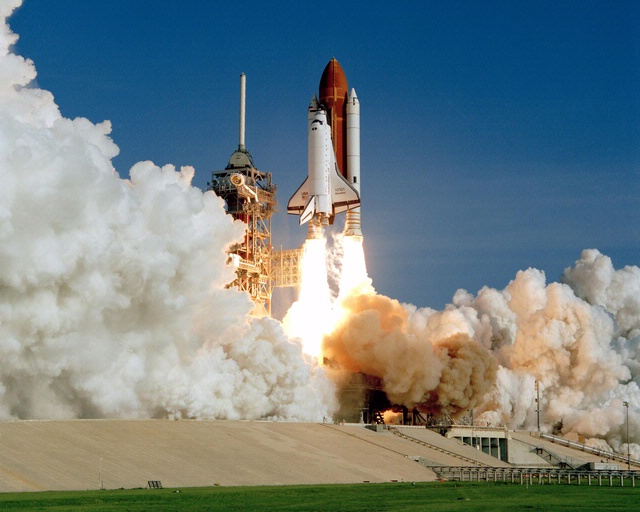
\includegraphics[scale=0.35]{gambar/roketluarangkasa.jpg}

  % Ubah sesuai dengan keterangan gambar yang diinginkan
  \caption{Peluncuran roket luar angkasa \emph{Discovery} \citep{roketluarangkasa}.}
  \label{fig:roketluarangkasa}
\end{figure}

Roket luar angkasa merupakan \lipsum[1]

\emph{Discovery}, Gambar \ref{fig:roketluarangkasa}, merupakan \lipsum[2]

\section{Gravitasi}
\label{sec:gravitasi}

Gravitasi merupakan \lipsum[1]

\subsection{Hukum Newton}
\label{subsec:hukumnewton}

Newton \citep{newton1687} pernah merumuskan bahwa \lipsum[1]
Kemudian menjadi persamaan seperti pada persamaan \ref{eq:hukumpertamanewton}.

% Contoh pembuatan persamaan
\begin{equation}
  \label{eq:hukumpertamanewton}
  \sum \mathbf{F} = 0\; \Leftrightarrow\; \frac{\mathrm{d} \mathbf{v} }{\mathrm{d}t} = 0.
\end{equation}

\subsection{Anti Gravitasi}
\label{subsec:antigravitasi}

Anti gravitasi merupakan \lipsum[1]

\cleardoublepage

% Bab 3 desain dan implementasi
\chapter{DESAIN DAN IMPLEMENTASI}
\label{chap:desainimplementasi}

% Ubah bagian-bagian berikut dengan isi dari desain dan implementasi

Penelitian ini dilaksanakan sesuai \lipsum[1][1-5]

\section{Deskripsi Sistem}
\label{sec:deskripsisistem}

Sistem akan dibuat dengan \lipsum[1-2]

\section{Implementasi Alat
  \label{sec:implementasi alat}}

Alat diimplementasikan dengan \lipsum[1]

% Contoh pembuatan potongan kode
\begin{lstlisting}[
  language=C++,
  caption={Program halo dunia.},
  label={lst:halodunia}
]
#include <iostream>

int main() {
    std::cout << "Halo Dunia!";
    return 0;
}
\end{lstlisting}

\lipsum[2-3]

% Contoh input potongan kode dari file
\lstinputlisting[
  language=Python,
  caption={Program perhitungan bilangan prima.},
  label={lst:bilanganprima}
]{program/bilangan-prima.py}

\lipsum[4]

\cleardoublepage

% Bab 4 pengujian dan analisis
\chapter{PENGUJIAN DAN ANALISIS}
\label{chap:pengujiananalisis}

% Ubah bagian-bagian berikut dengan isi dari pengujian dan analisis

Pada penelitian ini dipaparkan skenario pengujian yang dilakukan, termasuk kondisi lingkungan pengujian, perangkat keras dan perangkat lunak yang digunakan, serta parameter-parameter yang diuji. Informasi detail mengenai konfigurasi dan prosedur pengujian disajikan agar hasil pengujian dapat direplikasi dengan konsisten.

\section{Hasil Pengujian Performa Menggunakan Confusion Matrix}
\label{sec:hasilperformaconfisionMatrix}

Bagian ini membahas hasil pengujian performa deteksi objek menggunakan Confusion Matrix. Nilai seperti True Positive, True Negative, False Positive, dan False Negative dianalisis untuk menilai akurasi dan efektivitas deteksi.

\section{Pengujian Berdasarkan FPS}
\label{sec:pengujianberdasarkanfps}

Pengujian ini dilakukan untuk menganalisis kecepatan pemrosesan sistem dalam satuan Frame per Second (FPS). FPS yang tinggi menunjukkan bahwa sistem dapat bekerja dengan baik secara real-time. Grafik hasil pengujian disertakan untuk memudahkan visualisasi performa.

\section{Pengujian Berdasarkan Response Time}
\label{sec:pengujianberdasarkanresponsetime}

Bagian ini mengukur waktu yang dibutuhkan sistem untuk merespons setiap perubahan lingkungan atau perintah yang diterima. Response Time sangat penting untuk mengukur responsivitas sistem dalam skenario dinamis.

\section{Pengujian Kesesuaian Jarak Deteksi}
\label{sec:pengujiankesesuaianjarakdeteksi}

Pengujian dilakukan untuk mengukur kemampuan sistem dalam mendeteksi objek pada berbagai jarak, yaitu 150 cm, 100 cm, dan 50 cm. Setiap subbagian akan menjelaskan hasil pengujian dan menganalisis performa sistem pada jarak-jarak tersebut.

\subsection{Pengujian Kesesuaian Jarak Deteksi 150 cm}
\label{sec:pengujiankesesuaianjarakdeteksi150cm}

Hasil pengujian pada jarak 150 cm dianalisis untuk melihat kemampuan deteksi pada jarak jauh.

\subsection{Pengujian Kesesuaian Jarak Deteksi 100 cm}
\label{sec:pengujiankesesuaianjarakdeteksi100cm}

Pada jarak 100 cm, sistem diuji untuk mengetahui seberapa baik model bekerja pada jarak menengah.

\subsection{Pengujian Kesesuaian Jarak Deteksi 50 cm}
\label{sec:pengujiankesesuaianjarakdeteksi50cm}

Pengujian pada jarak 50 cm menunjukkan kemampuan deteksi pada jarak dekat dan tantangan yang mungkin dihadapi.

\section{Performa Keberhasilan Tracking}
\label{sec:performakeberhasiltracking}

Bagian ini mengevaluasi keberhasilan sistem dalam melakukan tracking terhadap objek target. Tingkat keberhasilan dianalisis untuk mengetahui keandalan sistem dalam berbagai skenario.

\section{Performa Akurasi Mengikuti Objek}
\label{sec:performaakurasiobjek}

Analisis dilakukan untuk mengukur seberapa akurat sistem dapat mengikuti objek target, termasuk mempertahankan jarak yang tepat dan tidak kehilangan objek dalam berbagai kondisi.

\section{Performa Keberhasilan Mengikuti saat Belok Kiri}
\label{sec:performabelokkiri}

Bagian ini membahas kemampuan sistem dalam mengikuti objek saat berbelok ke kiri. Tantangan yang dihadapi dan solusi yang diterapkan diuraikan.

\section{Performa Keberhasilan Mengikuti saat Belok Kanan}
\label{sec:performabelokkanan}

Bagian ini membahas kemampuan sistem dalam mengikuti objek saat berbelok ke kanan, mirip dengan bagian sebelumnya.

\section{Performa Keberhasilan Mengikuti Lajur Khusus}
\label{sec:performalajurkhusus}

Bagian ini menguji apakah sistem dapat mengikuti objek pada lajur khusus, seperti jalur sempit atau berbelok yang membutuhkan manuver khusus.

\section{Pembahasan Hasil}
\label{sec:pembahasanhasil}

Bagian ini membahas hasil-hasil pengujian secara keseluruhan dan memberikan insight mengenai performa sistem.

\subsection{Performa Deteksi Objek}
\label{sec:performadeteksiobjek}

Bagian ini menjelaskan kekuatan dan kelemahan deteksi objek yang ditemukan selama pengujian.

\subsection{Kecepatan Pemrosesan (FPS)}
\label{sec:kecepatanpemrosesan}

Menganalisis kecepatan pemrosesan secara keseluruhan dan pengaruhnya terhadap performa sistem real-time.

\subsection{Response Time}
\label{sec:responsetime}

Membahas hasil pengujian response time dan faktor-faktor yang mempengaruhi waktu respons.

\subsection{Kesesuaian Jarak Deteksi}
\label{sec:kesesuaianjarak}

Diskusi tentang performa sistem dalam mendeteksi objek pada berbagai jarak yang telah diuji.

\subsection{Performa Keberhasilan Tracking}
\label{sec:performatracking}

Membahas tingkat keberhasilan sistem dalam melacak objek dan kondisi yang mempengaruhi performa.

\subsection{Performa Akurasi Mengikuti Objek}
\label{sec:akurasiikutiobjek}

Evaluasi akurasi dalam mengikuti objek target, termasuk kondisi yang dapat menyebabkan kegagalan.

\subsection{Performa Keberhasilan Mengikuti}
\label{sec:keberhasilanmengikuti}

Menguraikan keberhasilan sistem dalam mengikuti objek saat menghadapi belokan dan lajur khusus.
\cleardoublepage

% Bab 5 penutup
\chapter{PENUTUP}
\label{chap:penutup}

% Ubah bagian-bagian berikut dengan isi dari penutup

\section{Kesimpulan}
\label{sec:kesimpulan}

Berdasarkan hasil pengujian yang \lipsum[1][1-3] sebagai berikut:

\begin{enumerate}[nolistsep]

  \item Pembuatan \lipsum[2][1-3]

  \item \lipsum[2][4-6]

  \item \lipsum[2][7-10]

\end{enumerate}

\section{Saran}
\label{chap:saran}

Untuk pengembangan lebih lanjut pada \lipsum[1][1-3] antara lain:

\begin{enumerate}[nolistsep]

  \item Memperbaiki \lipsum[2][1-3]

  \item \lipsum[2][4-6]

  \item \lipsum[2][7-10]

\end{enumerate}

\cleardoublepage

\chapter*{DAFTAR PUSTAKA}
\addcontentsline{toc}{chapter}{DAFTAR PUSTAKA}
\renewcommand\refname{}
\vspace{2ex}
\renewcommand{\bibname}{}
\begingroup
\def\chapter*#1{}
\printbibliography
\endgroup
\cleardoublepage

% Biografi penulis
\begin{center}
  \Large
  \textbf{BIOGRAFI PENULIS}
\end{center}

\addcontentsline{toc}{chapter}{BIOGRAFI PENULIS}

\vspace{2ex}

\begin{wrapfigure}{L}{0.3\textwidth}
  \centering
  \vspace{-3ex}
  % Ubah file gambar berikut dengan file foto dari mahasiswa
  
\includegraphics[width=0.3\textwidth]{gambar/elon.jpg}
  \vspace{-4ex}
\end{wrapfigure}

% Ubah kalimat berikut dengan biografi dari mahasiswa
\name{}, lahir pada \lipsum[1]

\lipsum[2]

\cleardoublepage

\end{document}
